
%|  Name  | TODO | ONGOING | DONE |
%|--------|------|---------|------|
%| Dana   | x    |         |      |
%| Gerd   |      |         | x    |
%| Glenn  | v    |         |   x  |
%| Jordan | x    |         |      |
%| Luke   | x    |         |      |
%| Matt   |      |         |  x   |
%| Neil   | x    |         |      |
%| Scot   | x    |         |   x   |

%CLEANUP \todo[inline]{Owner: Gerd -- Priority: High -- Effort: M -- Completion: 100\%}

Throughout this tour, we describe the life cycle of HDF5 files.

\paragraph{Terminology.} As we saw in the previous tour (Section~\ref{chap:hdf5-lib}), the term ``HDF5 library" has several context-dependent meanings. Likewise, the term `HDF5 file' refers to one of the following:

\begin{enumerate}
    \item A kind of HDF5 virtual object.
    \item A portion of the HDF5 library that represents an open HDF5 file.
    \item A terminal VOL connector-specific in-storage representation, including ``file-less."
    \item One or more files stored in a file system or object store formatted according to the HDF5 file format specification~\cite{ffmt}.
    \item A combination of one or more of the above, in a generic sense.
\end{enumerate}

We first describe an HDF5 file’s runtime life cycle before covering a few finer points in subsequent sections.

\subsection{Life cycle}

In this section, we describe the internals of an HDF5 file's life cycle, including VOL connector and VFD selection and handling, by reviewing the \texttt{H5Fcreate, H5Fopen,} and \texttt{H5Fclose} stacks. At the end of this section, the reader should have enough information to answer the following questions:

\begin{itemize}
    \item How do HDF5 library API calls get ``routed" through the VOL layer?
    \item Under what circumstances do they enter the native VOL connector?
    \item How are HDF5 files represented in memory?
    \item What is the HDF5 virtual file layer (VFL), and how does it relate to the rest of the HDF5 library?
    \item How does the HDF5 library select virtual file drivers (VFD)?
\end{itemize}

\paragraph{Prototype.} Let's consider the simplest program to create a new HDF5 file shown in Listing~\ref{lst:file-101}.

\begin{listing}
\centering
\caption{An ``empty'' (800 B) HDF5 file.}
\label{lst:file-101}
\begin{minted}[linenos]{C}
#include "common.h"
int main() {
    hid_t file_id = H5Fcreate("hello.h5", H5F_ACC_TRUNC, H5P_DEFAULTx2);
    H5Fflush(file_id, H5F_SCOPE_GLOBAL);
    size_t size;
    H5Fget_filesize(file_id, &size);
    printf("File size: %zu\n", size);
    H5Fclose(file_id);
    return 0;
}
\end{minted}
\end{listing}

We create an ``empty" HDF5 file. Of course, such a minimal HDF5 file must contain a root group! Finally, we print its in-storage size. (As we will see later, the call to \texttt{H5Flush} is necessary to get an accurate size.)

\paragraph{Goals.} The main goals of the HDF5 file creation/open/close life cycle are:
\begin{itemize}
    \item Create an in-memory representation of an HDF5 file.
    \item Return a file identifier or handle (\texttt{hid\_t}) to the caller.
    \item Serialize and persist the file object in storage.
    \item Free all resources associated with the file upon closure of the last handle.
\end{itemize}

\paragraph{Control flow.} As we saw in Section~\ref{chap:hdf5-lib}, any API call, in this case, \texttt{H5Fcreate}, will trigger library initialization, which includes the registration of the native VOL as the default VOL connector and the POSIX VFD (sec2) as the default file driver. 

The call sequence for each API routine used in Listing~\ref{lst:file-101} may be found in Figure~\ref{fig:tour2-file-create} (\texttt{H5Fcreate}), Figure~\ref{fig:tour2-file-flush} (\texttt{H5Fflush}), Figure~\ref{fig:tour2-file-get-filesize} (\texttt{H5Fget\_filesize}), and Figure~\ref{fig:tour2-file-close} (\texttt{H5Fclose}). For modules whose API functions are routed through the VOL layer, we have adopted the notion of top and bottom portions, e.g., \texttt{H5F Top} and \texttt{H5F Bot.} Since the HDF5 library modules predate the introduction of the VOL layer, the code is not neatly separated into VOL handling/native VOL code portions. We refer to a module's VOL handling code portions as the module's `top' portion and the native VOL portion as the module's `bottom.'

\texttt{H5Fcreate} enters the VOL layer at \texttt{H5VL\_file\_create} via \texttt{H5F\_\_create\_api\_common}. This routine handles sanity checking and calling the internal VOL layer routine, \texttt{H5VL\_file\_create}. The native VOL connector is selected, and its file creation callback, \texttt{H5VL\_\_native\_file\_create}, is invoked. The open routine from the file module, \texttt{H5F\_open}, does all the heavy lifting in terms of allocation and initialization of various in-memory structures (see the section on data flow), creates a metadata cache for the file under construction (\texttt{H5AC\_create}), and culminates in file superblock and root group creation.

On the following line, \texttt{H5Fflush} is routed through the VOL layer via \texttt{H5F\_\_flush\_api\_common}, which invokes the \texttt{H5VL\_file\_specific} callback with operation type \texttt{H5VL\_FILE\_FLUSH}. The flush operation is handled by the native VOL's \texttt{H5VL\_\_native\_file\_specific}.

Similarly, the call to \texttt{H5Fget\_filesize} is routed through the VOL layer's \texttt{H5VL\_file\_optional} callback with the operation type \texttt{H5VL\_NATIVE\_FILE\_GET\_SIZE}, eventually reaching the native VOL's implementation of the get filesize operation within \texttt{H5VL\_\_native\_file\_optional}. This invokes the native VOL's internal \texttt{H5F\_\_get\_max\_eof\_eoa}, which invokes the VFL's \texttt{H5FD\_get\_eo[a,f]} and adds them to the file's base address obtained from \texttt{H5FD\_get\_base\_addr}.

\texttt{H5Fclose} proceeds to decrement the file ID's reference count via \texttt{H5I\_dec\_app\_ref}. If the reference count has reached 1, which it has in this example, this triggers the invocation of the free function for the particular identifier type, a file ID (\texttt{H5I\_FILE}), in this case. The free function in this case is \texttt{H5F\_\_close\_cb} via which we re-enter the VOL through \texttt{H5VL\_file\_close}, which in turn calls the native VOL's \texttt{H5VL\_\_native\_file\_close}. This triggers the release of in-memory file resources, including flushing and destroying the file-specific metadata cache, via \texttt{H5F\_\_dest}.

\begin{comment} 
http://www.plantuml.com/plantuml/uml/
@startuml

participant "H5F Top" as H5Ft
participant H5VL as H5VL
participant "Native VOL" as native
participant "H5F Bot." as H5Fb

rnote over H5Ft: H5Fcreate
H5Ft -> H5VL: H5F__create_api_common
H5VL -> native: H5VL_file_create
native -> H5Fb: H5VL__native_file_create
H5Fb -> H5AC: H5F__open
rnote over H5AC: H5AC_create
rnote over H5Fb: H5F__super_init
participant "H5G Bot." as H5Gb
H5Fb -> H5Gb: H5G_mkroot

@enduml
\end{comment}

\begin{figure}
    \centering
    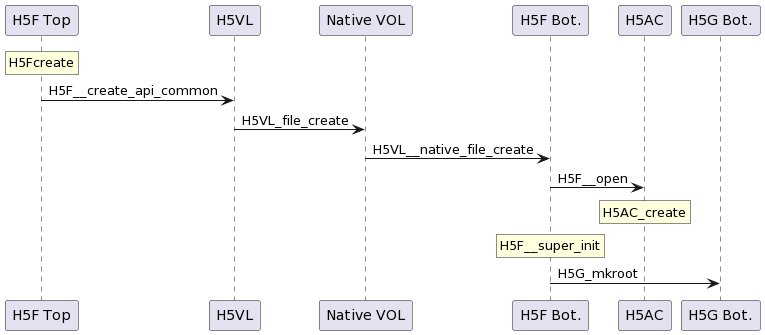
\includegraphics[width=0.80\textwidth]{images/tour2_file_create.png}
    \caption{File creation sequence diagram}
    \label{fig:tour2-file-create}
\end{figure}

\begin{comment}
http://www.plantuml.com/plantuml/uml/
@startuml

participant "H5F Top" as H5Ft
participant H5VL as H5VL
participant "Native VOL" as native
participant "H5F Bot." as H5Fb

rnote over H5Ft: H5Fflush
H5Ft -> H5VL: H5F__flush_api_common
H5VL -> native: H5VL_file_specific
native -> H5Fb: H5VL__native_file_specific
alt Global flush
rnote over H5Fb: H5F_flush_mounts
else Local flush
rnote over H5Fb: H5F_flush
end

@enduml
\end{comment}

\begin{figure}
    \centering
    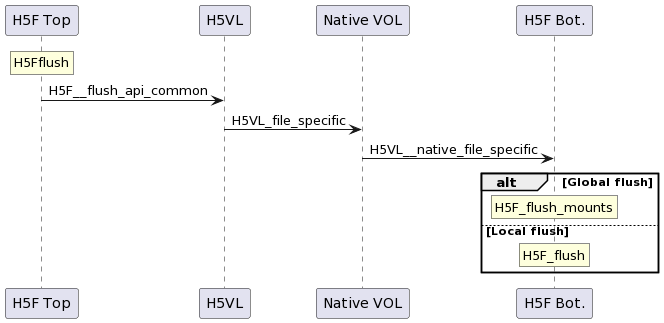
\includegraphics[width=0.7\textwidth]{images/tour2-file-flush.png}
    \caption{File flush sequence diagram}
    \label{fig:tour2-file-flush}
\end{figure}

\begin{comment}
http://www.plantuml.com/plantuml/uml/
@startuml
participant "H5F Top" as H5Ft
participant H5VL as H5VL
participant "Native VOL" as native
participant "H5F Bot." as H5Fb
participant H5FD
participant "sec2 Driver" as sec2

H5Ft -> H5VL: H5Fget_filesize
H5VL -> native: H5VL_file_otional
native -> H5Fb: H5VL__native_file_optional
H5Fb -> H5FD: H5F__get_max_eof_eoa
H5FD -> sec2: H5FD_get_eo[a,f]
rnote over sec2: H5FD__sec2_get_eo[a,f]
@enduml
\end{comment}

\begin{figure}
    \centering
    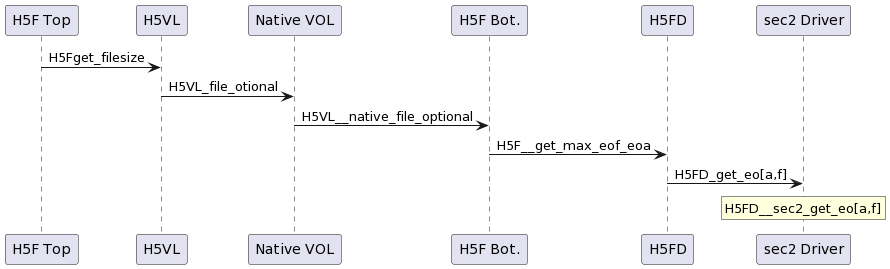
\includegraphics[width=0.95\textwidth]{images/tour2-file-get-filesize.png}
    \caption{Get filesize sequence diagram}
    \label{fig:tour2-file-get-filesize}
\end{figure}

\begin{comment}
http://www.plantuml.com/plantuml/uml/
@startuml
participant "H5F Top" as H5Ft
participant H5I as H5I
participant H5VL as H5VL
participant "Native VOL" as native
participant "H5F Bot." as H5Fb

H5Ft -> H5I:  H5Fclose
H5I -> H5Ft: H5I_dec_app_ref
H5Ft -> H5VL: H5F__close_cb
H5VL -> native: H5VL_file_close
native -> H5Fb: H5VL__native_file_close
rnote over H5Fb: H5F__dest
@enduml
\end{comment}

\begin{figure}
    \centering
    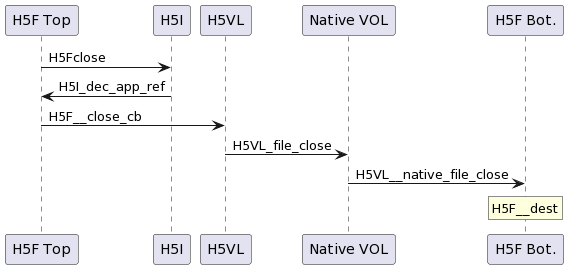
\includegraphics[width=0.70\textwidth]{images/tour2-file-close.png}
    \caption{File close sequence diagram}
    \label{fig:tour2-file-close}
\end{figure}

\begin{comment}
@startuml

participant Application as app
participant "H5F Top" as H5Ft
participant H5VL as H5VL
participant "Native VOL" as native
participant "H5F Bot." as H5Fb

app -> H5Ft: H5Fcreate
H5Ft -> H5Ft: H5F__create_api_common
H5Ft -> H5VL: H5VL_file_create
H5VL -> native: H5VL__native_file_create
native -> H5Fb: H5F__open
H5Fb -> H5AC: H5AC_create
H5Fb -> H5Fb: H5F__super_init
participant "H5G Bot." as H5Gb
H5Fb -> H5Gb: H5G_mkroot

app -> H5Ft: H5Fflush
H5Ft -> H5Ft: H5F__flush_api_common
H5Ft -> H5VL: H5VL_file_specific
H5VL -> native: H5VL__native_file_specific

app -> H5Ft: H5Fget_filesize
H5Ft -> H5VL: H5VL_file_otional
H5VL -> native: H5VL__native_file_optional
native -> H5Fb: H5F__get_max_eof_eoa
participant H5FD as H5FD
H5Fb -> H5FD: H5FD_get_eo[a,f]

app -> H5Ft: H5Fclose
participant H5I as H5I
H5Ft -> H5I: H5I_dec_app_ref
H5I -> H5Ft: H5F__close_cb
H5Ft -> H5VL: H5VL_file_close
H5VL -> native: H5VL__native_file_close
native -> H5Fb: H5F__dest

@enduml
\end{comment}

%\begin{figure}
%\centering
%\includegraphics[width=1\textwidth]%{images/tour_2_file_creation_and_size_retrieval.png}
%\caption{File creation and size retrieval sequence diagram.}
%label{fig:tour-2-uml-1}
%\end{figure}

Before looking at variants of this control flow, we look at the data flow and provide the ``Cliff notes" for the VOL and VFL layers. A detailed architectural overview can be found in Section~\ref{ref:vol}.

\paragraph{Data flow.} Every time \texttt{H5F[create,open]} is called, a structure of type \texttt{H5F\_t} (see Listing~\ref{lst:file-top}) is allocated.

\begin{listing}
\centering
\caption{A top-level file descriptor.}
\label{lst:file-top}
\begin{minted}[linenos]{C}
struct H5F_t {
    char          *open_name;
    char          *actual_name;
    H5F_shared_t  *shared;
    H5VL_object_t *vol_obj;
    unsigned       nopen_objs;
    H5FO_t        *obj_count;
    bool           id_exists;
    bool           closing;
    struct H5F_t  *parent;
    unsigned       nmounts;
};
\end{minted}
\end{listing}

Since HDF5 files can be opened multiple times with different \texttt{hid\_t} handles in the same process, the in-memory file representation is split into \texttt{H5open} instance-specific top (\texttt{H5F\_t}) and shared bottom portions of type \texttt{H5F\_shared\_t}. Both \texttt{H5F\_t} and \texttt{H5F\_shared\_t} are defined in \texttt{H5Fpkg.h}. \texttt{H5F\_shared\_t} is too extensive to be reproduced here, but it contains all the information that is common among \texttt{H5Fopen} instances, including:

 \begin{itemize}
     \item VOL connector and VFD information
     \item The metadata cache for this file and its configuration
     \item Version information
     \item Open HDF5 objects in the file
     \item File space management configuration
     \item Various status information.
 \end{itemize}
We strongly encourage the reader to review the well-documented \texttt{H5F\_shared\_t} definition!
 
Notice that most fields in \texttt{H5F\_shared\_t} show the file system heritage and represent information related to persisting HDF5 files in a file system according to the file format specification~\cite{ffmt}. For example, the \texttt{sblock} field of \texttt{H5F\_shared\_t} (see Listing~\ref{lst:file-sblock}) matches almost verbatim the file format specification.

\begin{listing}
\centering
\caption{File superblock in-memory representation.}
\label{lst:file-sblock}
\begin{minted}[linenos]{C}
typedef struct H5F_super_t {
    H5AC_info_t cache_info;
    unsigned    super_vers;
    uint8_t     sizeof_addr;
    uint8_t     sizeof_size;
    uint8_t     status_flags;
    unsigned    sym_leaf_k;
    unsigned    btree_k[H5B_NUM_BTREE_ID];
    haddr_t     base_addr;
    haddr_t     ext_addr;
    haddr_t     driver_addr;
    haddr_t     root_addr;
    H5G_entry_t *root_ent;
} H5F_super_t;
\end{minted}
\end{listing}

This is our first time encountering the metadata cache (\texttt{H5AC} module). For now, it is essential to remember that there is one metadata cache instance for each HDF5 file in the sense of \texttt{H5F\_shared\_t}, and \texttt{H5F\_super\_t} is its first protected entry.

Until this point, everything happened in memory, and no ``real" I/O has occurred. Considering the overhead associated with frequent small I/O operations, this behavior is quite desirable. Ignoring ``raw" data I/O, metadata, such as the file superblock, will be written only on flush events, or when an HDF5 file (\texttt{H5F\_shared\_t}) is closed, and the associated metadata cache instance is destroyed (see \texttt{H5F\_\_dest}). Speaking roughly, metadata I/O happens less frequently as the direct consequence of API calls than as the result of metadata cache events, such as entry evictions.

The downside of this apparent de-correlation of in-memory metadata management and I/O adds a certain fragility to the state of an HDF5 file that's open in a modifying access mode. If an application terminates unexpectedly, the library may not get to persist modified portions of the file state. Future implementations might offer better protection against file corruption.

It is hard to overstate the central role of the metadata cache's role in the HDF5 native VOL, although that might not yet be apparent. We will have more to say about the metadata cache in subsequent tours.

\subsection{Detour: The Virtual Object Layer}\label{sec:vol}

\paragraph{Goals} The purpose of the Virtual Object Layer (VOL) is to decouple the HDF5 library's API and object abstractions from a particular storage implementation while requiring minimal change in how the API is used. It allows for independent, potentially user-defined VOL connectors to handle virtual object operations. A common use case for VOL connectors is to change how HDF5 files are stored, mapping an HDF5 file in memory to something other than a POSIX file in storage - for example, a collection of objects in an AWS S3 bucket. The VOL layer's capabilities are more general than just changing the implementation of storage - a connector can perform arbitrary operations (such as logging, caching, or mirroring) whenever a routine that is part of the VOL API is used.

\paragraph{VOL Architecture}  Figure~\ref{fig:vol-arch} shows how the VOL fits into the library's structure. Operations that deal with storage or virtual objects are part of the VOL API, which means that calls pass through one or more VOL connectors before reaching storage. There are two types of VOL connectors: pass-through connectors, which pass control flow to another connector after performing some operation, and terminal connectors, which do not pass on to another connector and are generally used to map objects to storage. 

Library functions which are a part of the VOL API internally call a function of the form \\ \texttt{H5*\_\_<operation>\_api\_common}, which routes the call to the VOL layer via \texttt{H5VL\_<operation>}. The VOL layer determines which connector to use by checking the property list that was passed as an argument to the original API call.

For example, with the default file access property list (FAPL) specified by \texttt{H5P\_DEFAULT}, the top level \texttt{H5Fopen} internally calls \texttt{H5F\_\_open\_api\_common}, which passes control to \texttt{H5VL\_file\_open}. Because the default FAPL specifies the native VOL connector, \texttt{H5VL\_file\_open} will invoke the native VOL's file open callback \texttt{H5F\_open} (note the underscore!), which opens an HDF5 file object from a locally-stored POSIX file. A VOL connector provides pointers to its callbacks in its \texttt{H5VL\_class\_t} struct. (See Section~\ref{ref:vol}.)

VOL connectors other than the native connector are distributed as plugins loaded into an application. There are three ways to load a connector: dynamic loading using environment variables, dynamic loading with API calls, and manual linking to the connector.

\paragraph{Dynamic Loading with Environment Variables} Dynamic loading with environment variables does not require rebuilding or modifying the application. However, it does not allow an application to load multiple VOL connectors.

At runtime, the library checks the environment variable \texttt{HDF5\_VOL\_CONNECTOR} for the name of a VOL connector to load. This name is case-sensitive and is specified manually by each connector - the DAOS VOL connector, for example, expects to be discovered under the name \texttt{daos}. 

If the VOL connector is not installed to a default system path, then the environment variable \texttt{HDF5\_PLUGIN\_PATH} must be used to specify the absolute path to the connector. Generally, this will be the \texttt{/lib} subdirectory of wherever the connector was installed.

If the VOL connector is successfully loaded through environment variables, the library's default property lists, accessed via the \texttt{H5P\_DEFAULT} macro, will tell the VOL layer to use the dynamically loaded connector.

\paragraph{Dynamic Loading via API calls}  One of \texttt{H5VL\_register\_by\_name} or \texttt{H5VL\_register\_by\_value} can be used to load the specified VOL connector as a plugin and assign it an \texttt{hid\_t} handle. \texttt{H5VL\_register\_by\_value} expects a VOL connector identifier, a unique number assigned to each registered VOL by the HDF Group. \texttt{H5VL\_register\_by\_name} generally expects the same name that would be provided to \texttt{HDF5\_VOL\_CONNECTOR}, though this may vary by connector. 

Once the connector has been registered and assigned an \texttt{hid\_t} handle, this handle may be provided to \texttt{H5Pset\_vol} to modify a FAPL, telling any VOL layer function that checks this FAPL to use the supplied connector.

\paragraph{Manual Linking} Linking a VOL connector requires modifying the source and build of the target application but provides more flexibility in how the connectors may be used. 

The requirements to link and use a connector are as follows:
\begin{itemize}
    \item Link to the connector's library at application build time
    \item Include the connector's public headers in the application
    \item Potentially invoke any initialization/termination functions of the connector at the start/end of the application
\end{itemize}

Once these requirements are satisfied, the connector should provide a call of the form \texttt{H5Pset\_fapl\_<vol\_name>} or \texttt{H5Pset\_<vol\_name>} which modifies a FAPL, so that any VOL API calls provided with that FAPL will use the specified connector. Note that the exact function name for this operation will vary by connector in a way that does not adhere to any strict pattern.

\subsection{Detour: The Virtual File Layer}\label{sec:vfl}

A popular metaphor refers to HDF5 files as ``file systems in a file." The Virtual File Layer (VFL) adds some credibility to this metaphor. This section reviews the HDF5 Virtual File Layer, its requirements and assumptions, and its place in the library.

\paragraph{Overview} The VFL serves a purpose similar to the VOL -- outsourcing the implementation of specific storage-related operations to potentially user-defined Virtual File Drivers (VFDs) while minimizing the changes necessary in user applications. However, the scope of the VFL is narrower: it defines a mapping between the HDF5 address space and file system-like storage. 

As seen in Figure~\ref{fig:vol-arch}, the Virtual File Layer (VFL) sits at the bottom of the native VOL. It is a native VOL extension interface. If a non-native VOL is used, the VFL will be bypassed entirely. Just as the native VOL is the default VOL connector, the sec2 driver (or 'POSIX VFD') is the default VFD, which uses POSIX functions to perform unbuffered I/O (with respect to the HDF5 library) to a single file. (See Section~\ref{sec:H5PB} for a configuration in which the HDF5 library performs buffering.)

\paragraph{Using a VFD.} Unlike the VOL layer, which has only the native VOL built into the library, several VFDs are included with the library and can be enabled with build options. These include the MPI-IO VFD for parallel file access and the read-only S3 (ROS3) VFD, which allows read-only access to HDF5 files stored as objects in AWS S3 buckets.

The process of using a VFD that is not built with the library is similar to the process of using a manually linked VOL connector:
\begin{itemize}
    \item The VFD must be linked to the application at the application's build time
    \item The VFD's public headers must be included 
\end{itemize}

Once these requirements are satisfied, one of \texttt{H5Pset\_driver\_by\_name} or \texttt{H5Pset\_driver\_by\_value} may be used to modify a FAPL to enable use of the VFD. \texttt{H5Pset\_driver\_by\_name} requires a case-sensitive name specific to each VFD, and \texttt{H5Pset\_driver\_by\_value} requires a `driver value,' a unique number assigned to each VFD that is registered with The HDF Group.

Alternatively, each VFD should define a function with a name of the form \texttt{H5P\_set\_fapl\_<VFD\_name>}, which also modifies a FAPL to specify the use of that VFD. Listing~\ref{lst:file-core-vfd} shows a function of this form being used to enable the core VFD, a VFD that manages HDF5 files as contiguous memory buffers and maps I/O operations to memory accesses.

\paragraph{VFL Architecture.} Recall from the section on VOL Architecture that the property list for an operation determines which VOL is used. If the native VOL is selected, the property list also contains information about which file driver to use. Continuing the earlier example, the top level \texttt{H5Fopen} eventually calls the native VOL's \texttt{H5F\_open}, which invokes the VFL's \texttt{H5FD\_open}. This VFL function uses the 'open' callback of the active file driver, which for the default sec2 driver is \texttt{H5FD\_\_sec2\_open}. This driver callback is where the actual work to open a file in memory is performed. 

Each file driver provides pointers to its callbacks in an \texttt{H5FD\_class\_t} struct. These callbacks are invoked by handler functions with names of the form \texttt{H5FD\_<operation>} in the VFL layer. % See section~\ref{ref:vfl} for more information about the VFL.

\paragraph{Variants.} Signaling the presence of architecture (!), the two variants shown in Listings~\ref{lst:file-101-latest} and~\ref{lst:file-core-vfd} follow the same sequence that's shown in Figures~\ref{fig:tour2-file-create} through \ref{fig:tour2-file-close}. They diverge from the prototype (Listing~\ref{lst:file-101}) in only two minor technical details.

The code shown in Listing~\ref{lst:file-101-latest} will modify the default values of the \texttt{[low,high]\_bound} fields of the file's \texttt{H5F\_shared\_t} structure. This affects how certain file metadata is serialized (a process triggered by metadata cache events) if a newer file format specification offers better alternatives or a use case requires it.

\begin{listing}
\centering
\caption{A modern ``empty'' (195 B) HDF5 file.}
\label{lst:file-101-latest}
\begin{minted}[linenos]{C}
#include "common.h"
int main() {
    hid_t fapl_id = H5Pcreate(H5P_FILE_ACCESS);
    H5Pset_libver_bounds(fapl_id, H5F_LIBVER_LATEST, H5F_LIBVER_LATEST);
    hid_t file_id = H5Fcreate("my_file.h5", H5F_ACC_TRUNC, H5P_DEFAULT,
        fapl_id);
    H5Fflush(file_id, H5F_SCOPE_GLOBAL);
    size_t size;
    H5Fget_filesize(file_id, &size);
    printf("File size: %zu\n", size);
    H5Fclose(file_id);
    H5Pclose(fapl_id);
    return 0;
}
\end{minted}
\end{listing}

As described earlier, the code in Listing~\ref{lst:file-core-vfd} instructs the library to select a non-default VFD. This will update the \texttt{lf} field of the file's \texttt{H5F\_shared\_t} structure, which wraps the VFD-specific callbacks. In other words, only \texttt{H5FD\_*} calls will be affected by this change.

\begin{listing}
\centering
\caption{Using a different VFD.}
\label{lst:file-core-vfd}
\begin{minted}[linenos]{C}
#include "common.h"
int main() {
    hid_t fapl_id = H5Pcreate(H5P_FILE_ACCESS);
    H5Pset_fapl_core(fapl_id, 4096, 1);
    hid_t file_id = H5Fopen("my_file.h5", H5F_ACC_RDWR, fapl_id);
    size_t size;
    H5Fget_filesize(file_id, &size);
    printf("File size: %zu\n", size);
    H5Idec_ref(file_id);
    H5Idec_ref(fapl_id);
    return 0;
}
\end{minted}
\end{listing}

\subsection{Summary}

\begin{comment}
http://www.plantuml.com/plantuml
@startuml
participant "H5F Top" as h5ftop
participant H5VL as H5VL
participant "Native VOL" as native
participant "H5F Bot." as h5fbot
participant H5FD as H5FD
participant "Other VFD" as other_vfd
participant "Other VOL" as other_vol

h5ftop -> H5VL: H5Fcreate
rnote over H5VL: H5VL_file_open

alt Using Native VOL
 H5VL -> h5fbot: H5VL__native_file_open
 h5fbot -> H5FD: H5F_open
 rnote over H5FD: H5FD_open
alt Using sec2 driver
 rnote over H5FD: H5FD__sec2_open
 H5FD -> h5ftop: File open complete
else Using other VFD
 H5FD -> other_vfd: VFD open callback
end
else Using other VOL
 H5VL -> other_vol: VOL open callback
end
@enduml
\end{comment}

\begin{figure}
\centering
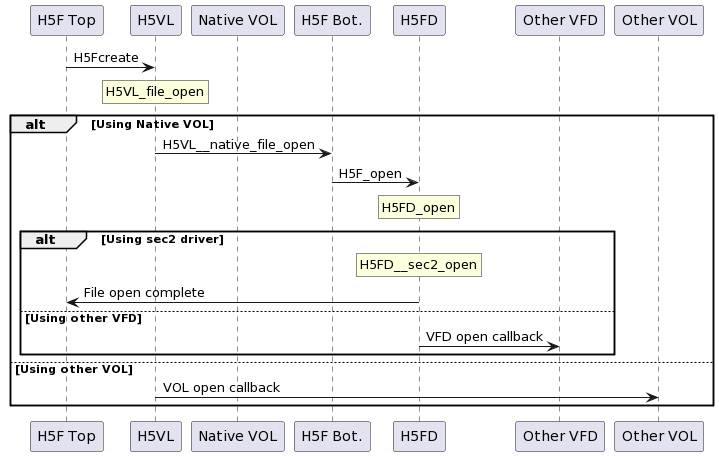
\includegraphics[width=0.80\textwidth]{images/tour-2-uml-vol.png}
\label{fig:tour-2-uml-vol}
\caption{File open through VOL and VFL sequence diagram}
\end{figure}

During this tour, we saw the interplay between the API, the Virtual Object Layer, the native VOL connector, and the Virtual File Layer. We saw how and which API calls are ``routed" through the VOL layer, which is perhaps the most important takeaway. We got a glimpse of how HDF5 files are represented in memory. Along the way, we encountered the metadata cache as one of the central architectural elements of the current library implementation. There is one metadata cache instance per HDF5 file, and rather than being directly controlled by API calls, metadata I/O occurs around metadata cache events indirectly triggered by API calls. While improving overall I/O performance, the ``split nature" of the state of a modified open HDF5 file makes it more vulnerable to unexpected application termination.

With extension interfaces such as VOL and VFD, the HDF5 library's extensibility is apparent but may make the simple creation of an HDF5 file appear overly complicated. However, very few applications stop at creating empty HDF5 files, and we saw some of the benefits of this when examining variants of the empty HDF5 file creation prototype.

During the next tour, we will examine how the HDF5 library handles user (meta-)data.